% Greedy Vitali selection: four open intervals, the two that are kept, and the triples.
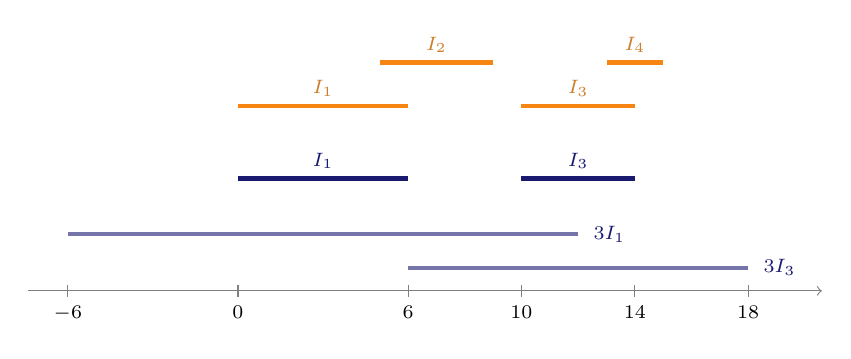
\begin{tikzpicture}[x=0.36cm,y=0.92cm]
  \draw[black!50,->] (-7.4,0) -- (20.6,0);
  \foreach \x/\lab in {-6/-6,0/0,6/6,10/10,14/14,18/18}{
    \draw[black!50] (\x,0.08) -- (\x,-0.08);
    \node[font=\scriptsize,below] at (\x,-0.08) {$\lab$};
  }
  \draw[BurntOrange,line width=1.7pt] (0,2.55) -- (6,2.55);
  \draw[BurntOrange,line width=1.7pt] (5,3.15) -- (9,3.15);
  \draw[BurntOrange,line width=1.7pt] (10,2.55) -- (14,2.55);
  \draw[BurntOrange,line width=1.7pt] (13,3.15) -- (15,3.15);
  \node[font=\scriptsize,BurntOrange!80!black,above] at (3,2.55) {$I_1$};
  \node[font=\scriptsize,BurntOrange!80!black,above] at (7,3.15) {$I_2$};
  \node[font=\scriptsize,BurntOrange!80!black,above] at (12,2.55) {$I_3$};
  \node[font=\scriptsize,BurntOrange!80!black,above] at (14,3.15) {$I_4$};
  \draw[MidnightBlue,line width=2.1pt] (0,1.55) -- (6,1.55);
  \draw[MidnightBlue,line width=2.1pt] (10,1.55) -- (14,1.55);
  \node[font=\scriptsize,MidnightBlue,above] at (3,1.55) {$I_1$};
  \node[font=\scriptsize,MidnightBlue,above] at (12,1.55) {$I_3$};
  \draw[MidnightBlue!60,line width=1.35pt] (-6,0.78) -- (12,0.78);
  \draw[MidnightBlue!60,line width=1.35pt] (6,0.32) -- (18,0.32);
  \node[font=\scriptsize,MidnightBlue,anchor=west] at (12.2,0.78) {$3I_1$};
  \node[font=\scriptsize,MidnightBlue,anchor=west] at (18.2,0.32) {$3I_3$};
\end{tikzpicture}
